\documentclass{article}
\usepackage{float}
\usepackage{amsmath,amssymb,amsthm,graphicx}
\usepackage{subcaption}
\usepackage{mleftright}
\graphicspath{ {./Images/} }

\setlength{\oddsidemargin}{0.25 in}
\setlength{\evensidemargin}{-0.25 in}
\setlength{\topmargin}{-0.6 in}
\setlength{\textwidth}{6.5 in}
\setlength{\textheight}{8.5 in}
\setlength{\headsep}{0.75 in}
\setlength{\parindent}{0 in}
\setlength{\parskip}{0.1 in}

\newtheorem{theorem}{Theorem}
\newtheorem{corollary}{Corollary}
\newtheorem{proposition}{Proposition}
\newtheorem*{remark}{Remark}
\theoremstyle{definition}
\newtheorem{example}{Example}
\newtheorem{definition}{Definition}

\newcommand{\lecture}[4]{
   \pagestyle{myheadings}
   \thispagestyle{plain}
   \newpage
%   \setcounter{lecnum}{#1}
   \setcounter{page}{1}
   \noindent
   \begin{center}
   \framebox{
      \vbox{\vspace{2mm}
    \hbox to 6.58in { {\bf CSC~565: Graph Theory
                        \hfill North Carolina State University} }
    \hbox to 6.58in { {\bf Fall 2019
                        \hfill Computer Science} }
       \vspace{4mm}
       \hbox to 6.28in { {\Large \hfill Lecture #1: #2  \hfill} }
       \vspace{2mm}
       \hbox to 6.28in { {\it Lecturer: {\it Don Sheehy {\tt <drsheehy@ncsu.edu>}} \hfill Scribe: #4} }
      \vspace{2mm}}
   }
   \end{center}
   \markboth{Lecture #1: #2}{Lecture #1: #2}
   \vspace*{4mm}
}


\begin{document}
    \lecture{25}{Nov 18, 2019}{}{Niranj Jyothish, Xun Jia}

    \section{Incidence Matrix as a Graph Representation}
    
    A graph can be represented as a matrix which represents it as mapping from edges to vertices. This form of a matrix is called an Incidence Matrix (B).
    
     $$B =
    \left[ {\begin{array}{cccc}
    	. & 1 & . \\
    	. & 0 & .\\
    	. & 0 & .\\
    	. & 1 & . \\
    	\end{array} } \right]
    $$  
    
    Lets say, the $k^{th}$ column has the ones at $i^{th}$ and $j^{th}$ row. 
    This form represents edge, $e_{k} = ( v_{i},v_{j})$
    
    B $\in \{0,1\}^{n\times m}$ where n is number of vertices and m is edges.
    
    B : $\{0,1\}^n -> \{0,1\}^m$ 
    
    Also written as, Pow(E) $->$ Pow(V).  Set of edges to vertices. 
   
    
    Lets say, $u \subseteq V$ which implies  $u \in \{ 0,1 \}^{n}$ 
    
    $$u_{i} =
    \left\{
    \begin{array}{ll}
    1\hspace{1cm} if  v_i \in u\\
    0\hspace{1cm} o/w\\
    \end{array}
    \right.$$
    
    And $X \subseteq E$ which implies $X \in \{0,1\}^m$
    
    Note: Multigraphs can be represented using Incidence Matrix but cannot represented by Adjacency Matrix.
    
    
    
    \section{Kernel of a Graph}
  	
  	Lets think of a new operation. We know in an incidence matrix, B , $e_{i} = (v_{j},v_{k})$
  	
  	$B[1]i = 
		   \left[ {\begin{array}{cccccccc}
		  	1  \\
		  	.  \\
		  	.  \\
		  	1  \\
		  	\end{array} } \right]
	  	\text{1s at } j^{th} \text{ and } k^{th} \text{ row}
	$
	
	This implies $Be_i = v_j + v_k$
    
    Example: Figure 1 
    
	$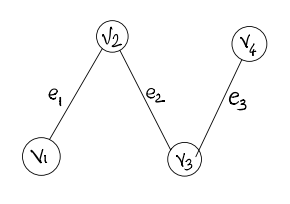
\includegraphics[width=0.3\textwidth]{p1.png}$
    	
    From figure 1,
 	$B(e_1 + e_3) = Be_1 + Be_3$
    			 $= v_1 + v_2 + v_3 + v_4$
    
    $B(e_1 + e_2) = v_1 +v_2 + v_2 + v_3$
    			$ = v_1 + v_3 $
    			
    Lets say, there is a path from u to v. $ P \subseteq E$
    
    BP = u + v

	Let C be the edges of a cycles ! What is BC? BC = 0.
	
	Kernel, ker B = { v : Bv = 0 }
	
	$ u , v \subseteq kerB$ \newline
	B(u+v) Bu + Bv = 0 + 0 = 0
	
	Kernel is also called cycle space of G
	
	\subsection{Extending idea of kernels to cycle space}
	
	What if, we add two cycle graphs. What resultant graphs we can expect.
	
	Case 1: When egde sets of two cycle graphs are disjoint.
	
	$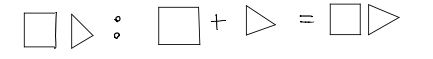
\includegraphics[width=0.5\textwidth]{p7_1.png}$
	
	
	We get the same graph.
	 
	Case 2: When edges set of two cycle graphs share an edge.

	$
\includegraphics[width=0.5\textwidth]{p7_2.png}$
		

	We get the cycle graphs glued.
	
	Find a case where, when two or more cycle in a graph gets added to form disjoint cycles.
	 
	$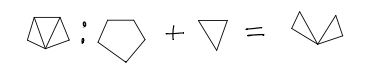
\includegraphics[width=0.5\textwidth]{p7_3.png}$
		
	$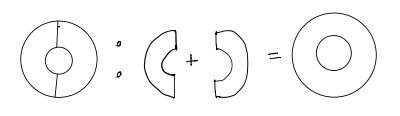
\includegraphics[width=0.5\textwidth]{p7_4.png}$

	Thus, the cycle space denoted by the basis of the graph not only gives an idea about the individual cycles in the graph but also, the addition of cycles.  
	
	Fact: Bounded faces of a 3-connected planar form a basis for kerB.
	
    
    \subsection{Using kernels to denote connectivity}
    
    Lets say we have a graph with $v_i, v_j \in V$
    
    We say it is connected , if there is a path $ P \subseteq E$ from $v_i$ to $v_j$
    
    We have seen earlier in the lecture about the behaviour of incidence matrix, B on paths. When we operate B on paths we just get the end points of a graph.Therefore,
    
    BP = $v_i$ + $v_j$
    
    $v_i$ = $v_j$ + BP
   
    \textbf{Image of B: } im B = $\{$ v : v = Bx for some x $\}$
    
	$v_i$ , $v_j$ are connected iff $v_i$ = $v_j$ + imB
	
	$v_i \in V$ ,  [$v_i$] = $v_i$ + imB
	
	Quotient vector space is denoted by :	 \newline
	V /imB $\cong$ connected components . [$v_i$] = [ $v_j$]
	
	[$v_i+v_j$ ] = $v_i$ + $v_j$ + imB = [$v_i$] + [$v_j$]
	
	Equality in V / imB is the same as connected in G.
	
	Example figure 2:
	
	$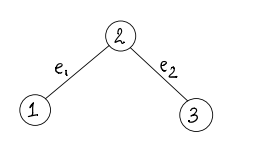
\includegraphics[width=0.35\textwidth]{p4.png}$

    $B = 
    \left[ {\begin{array}{cccccccc}
    	1  & 0\\
    	1 & 1  \\
    	0 & 1  \\
    	\end{array} } \right]
    $
    
    imB = $\{$ $\phi$ , $\{1,2\}$ , $\{2,3\}$ , $\{1,3\}$ $\}$

	Example figure 3:
		
	$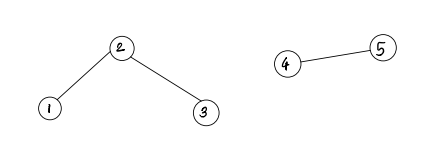
\includegraphics[width=0.5\textwidth]{p5.png}$
	
	imB = $\{$ $\phi$ , $\{1,2\}$ , $\{2,3\}$ , $\{1,3\}$, $\{4,5\}$ $\}$


\section{Another form of Incidence Matrix}

 $$\partial =
\left[ {\begin{array}{cccc}
	. & 1 & . \\
	. & 0 & .\\
	. & 0 & .\\
	. & -1 & . \\
	\end{array} } \right]
$$  

  Lets say, the $k^{th}$ column has the ones at $i^{th}$ and $j^{th}$ row. 
This form represents edge, $e_{k} = ( v_{i},v_{j})$

   $$\partial =
  \left\{
  \begin{array}{ll}
  1\hspace{1cm} \text{if } e_k = (v_i,v_j) i<j\\
  -1\hspace{1cm} \text{if } e_k = (v_i, v_j) i>j\\
  0\hspace{1cm} 0/w\\
  \end{array}
  \right.$$
  
  Example figure 4:
  
  	$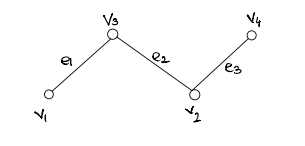
\includegraphics[width=0.5\textwidth]{p6.png}$
  
   $$\partial =
  \left[ {\begin{array}{cccc}
  	1 & 0 & 0 \\
  	0 & 1 & 1 \\
  	-1 & -1 & 0\\
  	0 & 0 &  -1 \\
  	\end{array} } \right]
  $$  
  
  $\partial (e_1 + e_2 + e_3)$ =  $$\partial =
  \left[ {\begin{array}{cccc}
  	 1\\
  	 1\\
  	 1\\
  	\end{array} } \right]
  $$  
  
  $ = (v_1 - v_3) + (v_2 - v_3) + (v_2 - v_4) = v_1 -2v_2 - 2v_3 - v_4$
  
  $\partial (e_1 - e_2 + e_3) = (v_1 - v_3) - (v_2 - v_3) + ( v_2 - v_4) = v_1 - v_4 $
  
  We looked at symmetric matrices and how wrangling matrices with its transpose gives symmetric matrices preserving properties and information.
  like rank of a matrix.
  
  Lets take $\partial$ and multiply with $\partial^T$.
   $\partial\partial^T$ $\in$ $R^{n \times n}$
  
  $[\partial \partial^T]_{ii} $ = $\sum_{j=1}^{m} \partial_{ij} \partial^T_{ji}$ = $\sum_{j=1}^m \partial_{ij}^2$ = deg($v_i$)
  
   $$\partial_{ij} =
  \left\{
  \begin{array}{ll}
  1\hspace{1cm} if  v_i \in u\\
  0\hspace{1cm} o/w\\
  \end{array}
  \right.$$ 
  
  $[\partial \partial^T]_{ik} $ = $\sum_{j=1}^{m} \partial_{ij} \partial^T_{jk}$ = $\sum_{j=1}^m \partial_{ij} \partial_{kj}$
  
  $$\partial_{ij} \partial_{kj} =
  \left\{
  \begin{array}{ll}
  -1\hspace{1cm} if  e_j=(v_i,v_k)\\
  0\hspace{1cm} o/w\\
  \end{array}
  \right.$$ 
  
  Therefore $\partial\partial^T$ is Laplacian Matrix.
  
  Also, Fact : ker ($\partial\partial^T$) $\cong $ connected components.
  
\end{document}